\documentclass{article}
\usepackage[backend=biber, style=authoryear-icomp]{biblatex}
\usepackage{blindtext}
\usepackage{multicol}
\usepackage[document]{ragged2e}
\usepackage[pass, letterpaper]{geometry}
\usepackage{amsmath}
\usepackage{amsfonts}
\usepackage{xcolor}
\usepackage{caption}
\usepackage{graphicx}
\usepackage{subcaption}
\addbibresource{ref.bib}

% Define macros
\newcommand\note[1]{\textbf{\textcolor{red}{#1}}}

% Captions
\captionsetup{justification = raggedright, singlelinecheck = false, labelfont=bf}

\title{Using a Deep Autoencoder Model to Characterize Air Pollution}
\author{Nicolas Shannon$^{1}$, Vandana Nunna Lakshmi$^{2}$}
\date{}
% To cite, use \parencite{} or \textcite{}

\begin{document}

% Acknowledgements
\begin{centering}
\maketitle
\vspace{-0.50cm}
\scriptsize
{$^{1}$Department of Computer Science, Loyola University Chicago, Chicago, IL, US}\\
{$^{2}$Department of Computer Science, University North Texas, Denton, TX, US}\\
%{$^{3}$Department of Electrical and Computer Engineering, University of Texas 
%    - Rio Grande Valley, Brownsville, TX, US \note{$\leftarrow$ fix formatting}}
\end{centering}

\begin{abstract}
Air pollutants are both a cause and a symptom of climate change. Global warming has the potential to raise
the levels of various air pollutants. The rise in surface air pollutants can lead to heat trapped close to 
the Earth's surface by virtue of the greenhouse effect, which further perpetuates the cycle. In order to
more effectively combat climate change, it is important to understand and characterize the source of 
emissions. We developed a technique to characterize cities by the levels of various air toxins using an
undercomplete autoencoder model. By representing the pollution levels of eighteen thousand cities across
the United States, we explore some of the more prominent features that characterize urban pollution.
We compare two techniques for reducing the input dimensionality - Principle Component Analysis (PCA) and
Undercomplete Autoencoders.
\end{abstract}

\vspace{0.25cm}
\section{Introduction}
Over the past several decades, air pollution has been a major concern for human health
and the environment. The EPA sets national air quality standards for  six major air
toxins: ground level Ozone (O$_3$), Carbon Monoxide (CO), Sulfur Dioxide (SO$_2$),
Lead (Pb), Nitrogen Dioxide (NO$_2$), and particulate matter (PM). \parencite{NAAQS09}.
The sources of these emissions vary, but the two largest contributors are industrial 
processes and motorized vehicles.

\newpage

Short and long term exposure to air toxins pose significant risk to human health. 
A study by \textcite{Wang19} found a correlation  between increased ambient CO
levels and outpatient visits for respiratory, cardiovascular, genitourinary, and gastrointenstinal
diseases. Several studies performed by the EPA also suggest that people with pre-existing health
conditions are at higher risk when exposed to CO over long periods.\par

\subsection{Air Toxins}
We wanted to explore how CO and other gases can be characterized with respect to location
in an effort to provide researchers and policy makers with the context and tools necessary to
make informed decisions. There are a litany of technologies and tools for pollution prevention
and control, but most of these options require contextual information and large amounts of data.
\par
By creating an embedding of time series pollution data for numerous cities throughout the U.S.,
we can explore the more interesting features of the model as well as apply it to tangential 
areas such as the pollution generated by industrial farming and animal husbandry activities.

\begin{figure}[h]
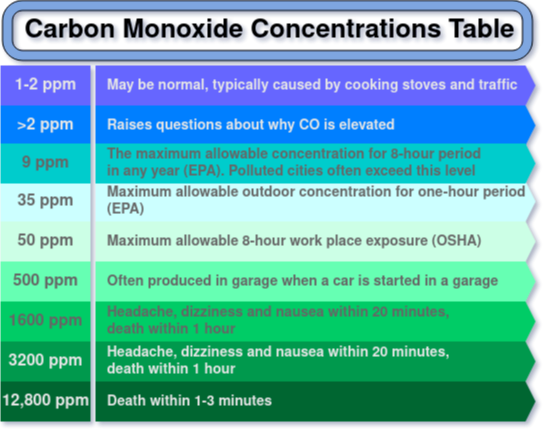
\includegraphics[width=\textwidth]{/home/nicks/github_repos/Pollution-Autoencoders/paper-draft/images/co-concentration-table.png}
    \caption{Carbon Monoxide Exposure Table, Parts Per Million (ppm)}
    \label{fig:co-exposure}
\end{figure}

\subsection{A Deep Learning Approach}
In this paper we employ autoencoder and  principle component analysis (PCA) models to 
feed the pollutant data and perform data compression. The resulting embeddings are 
compared in terms of effeciency and data loss. The features are encoded at different
scales of dimensions to check the fluctuation in explainable variance when predicting a 
given target. Given that each feature in the dataset represents the daily average of a 
specific pollutant in that location and that pollution levels do not vary drastrically 
on a day-to-day basis, it is evident that there is a strong correlation among features
\par While a healthy correlation among features is encouraged, abnormally strong values
relfect redundancy and end up being a burden on the model.
\parencite{featureredundancy}. First, deep autoencoders are better at compressing highly 
complex data into fewer dimensions. Autoencoders with a nonlinear encoder and decoder 
function can learn more powerful nonlinear generalizations than PCA. 
\parencite{Goodfellow16}.



\section{Related Work}
The idea of generating embeddings for a location is a highly potential expanse for
research. The two major forces behind its competency are, the fact that large volumes of
data is being effectively compressed and that these embeddings, when plugged into any
model could effectively represent any given location.  A lot of research is being done 
on location embeddings in recent times. For instance, location embeddings are being 
generated based on human-mobility data \parencite{GeoEmbeddings} to understand the 
behavioral proximity between different locations irrespective of their spatial distances.
The sequence of locations that are frequently travelled were fed to a Skip-gram Word2vec 
model to generate the location embeddings. Another approach that was implemented to 
leverage location embeddings is, GPS2Vec  \parencite{GPS2Vec}.  This application consists
of a neural network that would generate embeddings for a location, based on the semantic 
contexts that are sourced from the user content published on multiple digital platforms.
With the integration of these embeddings, a successful geo-tagged image classification 
task is demonstrated. In another effort  \parencite{PlaceDeduplication}, the location 
embeddings derived from user content such as addresses, phone numbers, images, place
names and all other details from multiple individual online posts, are compressed to 
form low dimensional embeddings to solve the place duplication issue. Deduplication of 
locations, is a paramount task for any digital platform since they provide a place graph
to its users, which is the result of merging location data from multiple sources. This 
merge leads to duplicity since different sources could hold different names for the same 
place. By applying K-NN search, pair-wise duplication prediction on these generated 
location embeddings, the application can identify the duplicates and eliminate them to 
result in an efficient place graph.\par
In 2018, a new approach, “DeepMove” is proposed \parencite{DeepMove}. This 
implementation employs Trip model and OD model to learn latent representations of 
places.  The approach is successfully applied to New York city yellow taxi dataset – 
“includes pick-up/drop-off times, the number of passengers, pick-up/drop-off locations 
represented by longitude and latitude, trip distance, rate types, payment type, and
itemized fares” \parencite{DeepMove}. Similarities among locations in New York city are 
derived effectively with “DeepMove”. To resolve the dissonance that arises from the 
fusion of geographic and semantic features of a location, an unsupervised learning 
implementation had been demonstrated that would derive location embeddings from human 
trajectories \parencite{DisentangledLocationEmbeddings}. With the ever- growing 
footprint of digital and social media platforms in everyday life of an individual, a
lot of research is happening to generate embeddings based on the content posted in 
different locations. LeGo-CM is one such effort that would generate embeddings of 
geotagged tweets \parencite{GeotaggedTweets}. These resultant embeddings could be 
applied to understand the kind of content each location reflects.Venue2Vec is another 
idea that is implemented to enhance the location-aware services in various platforms 
\parencite{Venue2Vec}. This model is trained on semantic data, temporal-spatial context 
and sequential relations among locations to generate embeddings. This makes sure that 
locations with similar data would fall close, when plotted in a multi-dimensional space,
based on the input features. Hence, the model is effective in predicting the next and  
future check-in location. Community Flow prediction is another area of interest where
embeddings are a major problem solver. Geo-contextual Multitask Embedding Learner (GMEL)
, is a model that uses “Graph Attention Network” to encode geographical contexts and 
spatial correlations to generate location embeddings \parencite{CommutingFlowPrediction}.
These embeddings are further used to predict the community fow that serves as a vital
factor in policy establishment and metro planning.


\section{Methodology}

We used two different methods to reduce the dimensionality of our data - Principle Component
Analysis and undercomplete autoencoders. A simple linear regression was performed on 
the encoded data that was generated by both the PCA and AE models. Additionally, we performed
a linear regression on the unencoded values for comparison. Each model's goodness of fit
was evaluated using the percentage of explained variance for the three linear regressions. 

% pipeline
\begin{figure}[h]
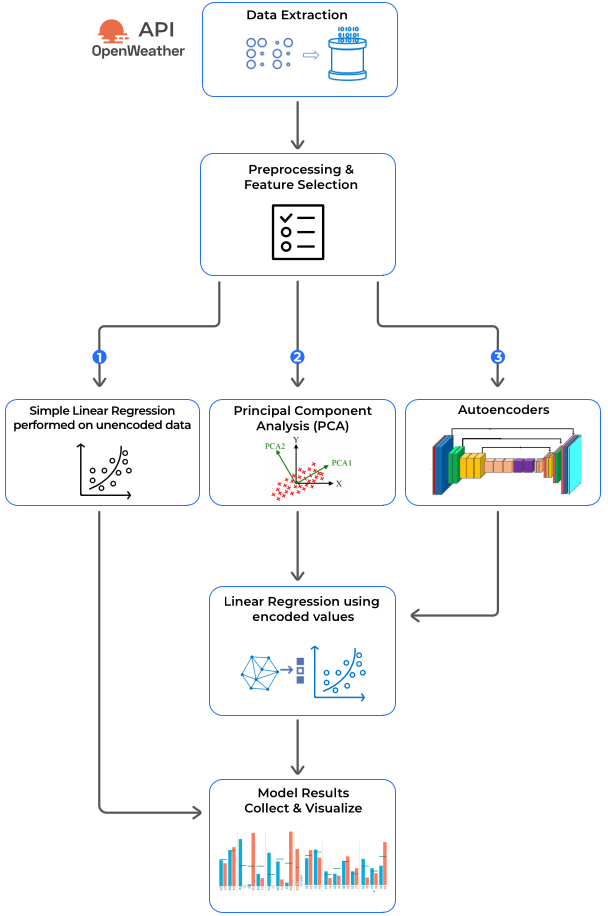
\includegraphics[width=\textwidth, height=6cm]{/home/nicks/github_repos/Pollution-Autoencoders/paper-draft/images/pipeline.png}
\caption{Data Pipeline}
\label{fig:pipeline}
\end{figure}

\subsection{Data Collection and Preprocessing}
The dataset was created using OpenWeather's Air Pollution API. The dataset includes data for 
eight polluting gases and particulates: CO, NO, NO$_2$, O$_3$, SO$_2$, NH$_3$, PM$_{2.5}$, 
and PM$_{10}$. The dataset also includes the hourly timestamp, the latitude and longitude (part of the input),
and the air quality index, the latter of which we did not end up using.\par
We looked at data for the eight pollutants over a six-and-a-half month time 
frame: January 27th, 2020 through June 6th, 2021. Our final 
dataset included just over eighteen thousand cities in the United States and other U.S. 
territories. We found it easier to focus on a single gas when developing 
the models, so we chose to concentrate on CO during the engineering process. Given
enough time and computational power, the techniques performed on the CO model would be 
easily extensible and transferable for the other seven pollutants.


% dataset characteristics table
\begin{table}[h!]
    \caption{Dataset Characteristics}
    \label{tab:table1}
    \vspace{0.1cm}
    \begin{tabular}{p{4cm}p{7cm}}
        \hline
        \multicolumn{2}{c}{OpenWeather Pollution API} \\
        \hline
        Sampling period  & 11/27/20 to 06/05/21\\
        Time interval & Daily  \\
        $\#$ of cities & 18,526 \\
        $\#$ of features & 191 \\
        $\#$ of component gases & 8 \\
        Dependent variable & Single day of time series (06/05/21) \\
        \hline
    \end{tabular}
\end{table}

OpenWeather's Pollution API ordinarily returns hourly values, but we opted to use the daily
average pollution levels as our feature set in order to make the number of starting dimensons
more manageable. We resolved to feature engineer the daily 
averages and proportional to the number of features and thus avoid the curse of dimensionality. 
\parencite{Trunk79}. \note{Idk about this} \par
We separated the dependent from the input before unit normalizing the input. 
The normalized data was then encoded by each model. 

\subsection{Undercomplete Autoencoder Model}
The autoencoder model used consists of an encoded and decoded layer. We performed
a grid search for the CO model to determine the optimal hyperparameters. The following 
hyperparameters were tested:
\begin{itemize}
    \item \textit{Learning Rate:} 0.0001, 0.001, 0.01, 0.1
    \item \textit{Batch Size:} 32, 64, 128, 256
    \item \textit{Epochs:} 10, 50, 75, 100
\end{itemize}
K-folds cross validation was used to validate the grid search using five folds. We selected the
highest coefficient of determination that appeared in each of the five folds for every given
dimension. The most frequently occuring combination of hyperparameters was then used to create
the finalized embedding.

\begin{table}[h!]
    \caption{Dataset Characteristics}
    \label{tab:table1}
    \vspace{0.1cm}
    \begin{tabular}{p{4cm}p{7cm}}
        \hline
        \multicolumn{2}{c}{Optimal Hyperparameters for Carbon Monoxide (CO)} \\
        \hline
        Activation function & tanh\\
        Loss function & Mean Squared Error  \\
        Optimizer & Adam \\
        Learning rate & 0.001 \\
        Batch size & 64 \\
        Epochs & 150 \\ 
        \hline
    \end{tabular}
\end{table}

\subsection{Principle Component Analysis}
The PCA model was trained with k-fold cross-validation using five folds. The dataset was
split into a training, validation, and hold-out test set.

\subsection{Model Validation}
K-folds cross validation was performed on the linear regression test using five folds. The folds
with the best and worst variance scores were extracted so as to make an equitable evaluation of
the model.

\section{Results}
We compared the percent explained variance across one hundred twenty dimensions for
the encoded values generated by the PCA and autoencoder models as well as for the unencoded
values by using a simple linear regression. While PCA was overall less noisy, we found that
the autoencoder model achieved a much higher explainable variance for the first few dimensions.
\\ \note{Note that results graphs are placeholders}
% ae vs pca linegraph
\begin{figure}[h!]

\begin{subfigure}{0.5\textwidth}
    \includegraphics[width=1.1\linewidth, height=4cm]{/home/nicks/github_repos/Pollution-Autoencoders/paper-draft/images/ae_all_dims.png} 
    \caption{Autoencoder Dimensionality Reduction}
    \label{fig:ae_dim_reduction}
\end{subfigure}% <- % sign must be here!
\begin{subfigure}{0.5\textwidth}
    \includegraphics[width=1.1\linewidth, height=4cm]{/home/nicks/github_repos/Pollution-Autoencoders/spaper-draft/images/ae_all_dims.png}
    \caption{PCA Dimensionality Reduction}
    \label{fig:pca_dim_reduction}
\end{subfigure}

\caption{Graph of autoencoder and PCA reduced representations of air pollutants}
\label{fig:ae_vs_pca}
\end{figure}

\par We clustered the cities based on the first two latent dimensions in order to see how
the model characterizes each city

% co scatter
\begin{figure}[h!]

\begin{subfigure}{0.5\textwidth}
    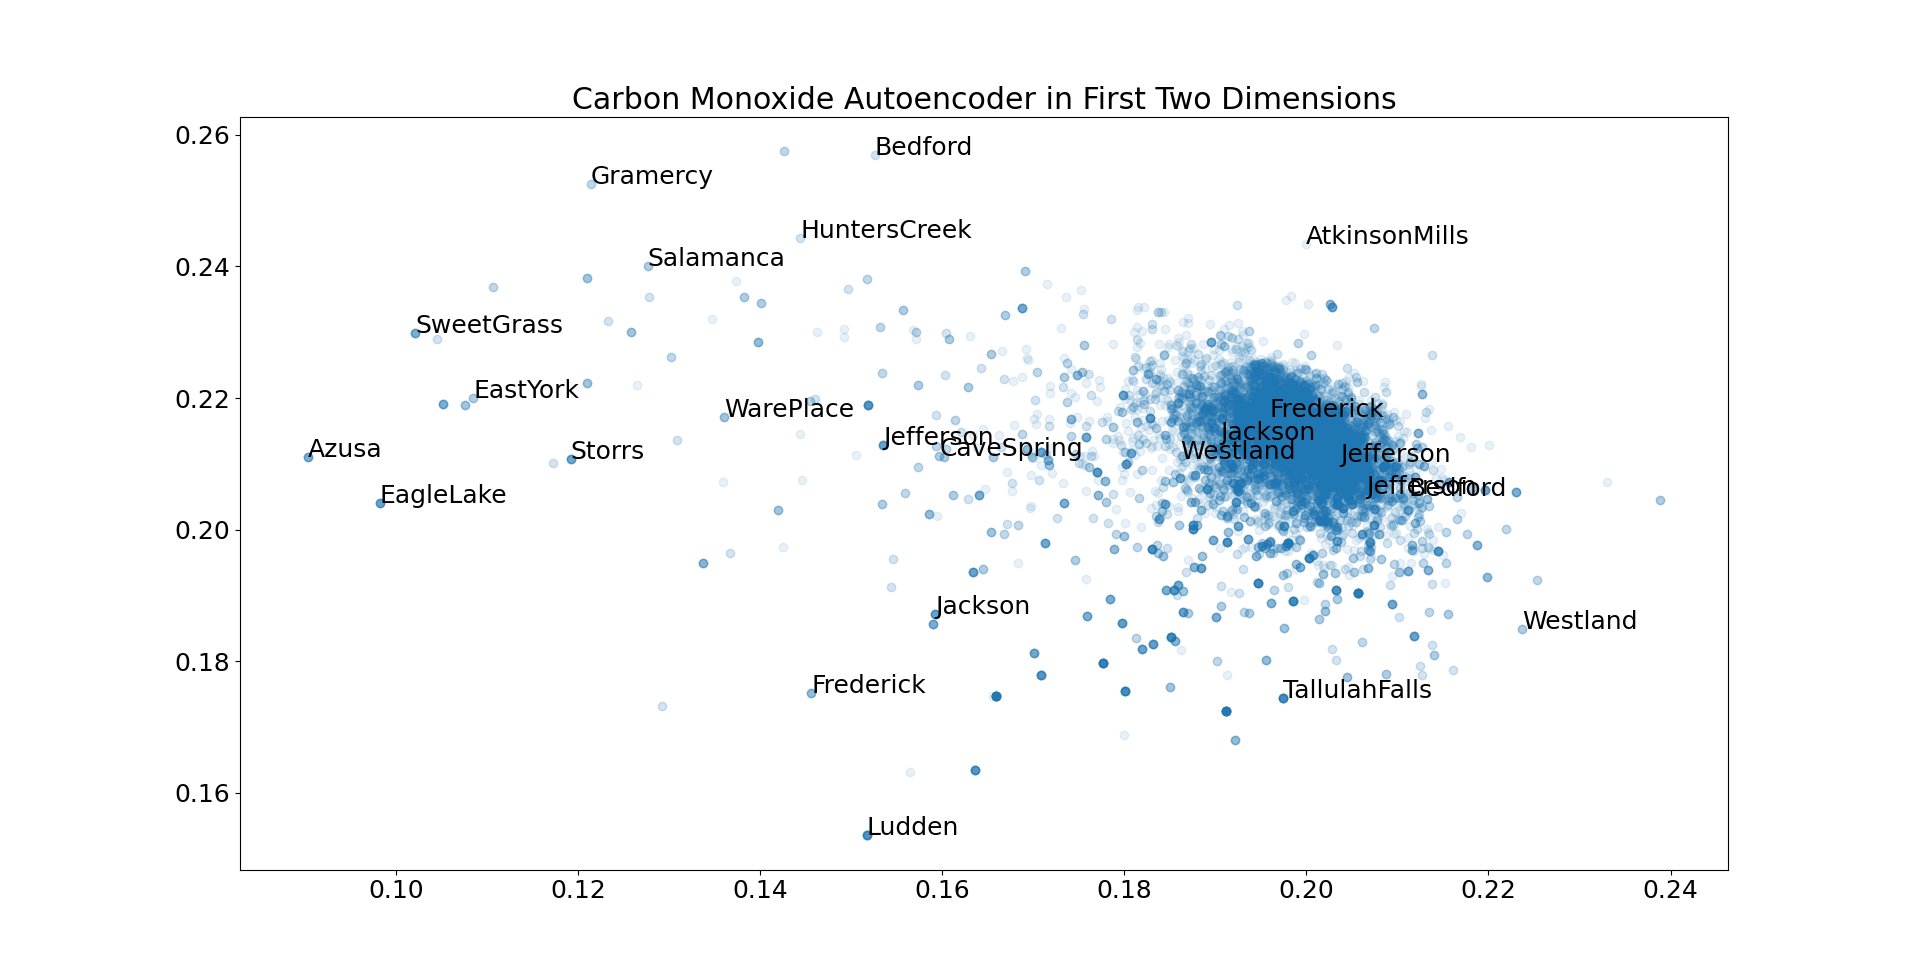
\includegraphics[width=1.1\linewidth, height=5cm]{/home/nicks/github_repos/Pollution-Autoencoders/paper-draft/images/co_scatter_ae_wlist.png} 
    \caption{Outlier Cities}
    \label{fig:outliers}
\end{subfigure}% <- % sign must be here!
\begin{subfigure}{0.5\textwidth}
    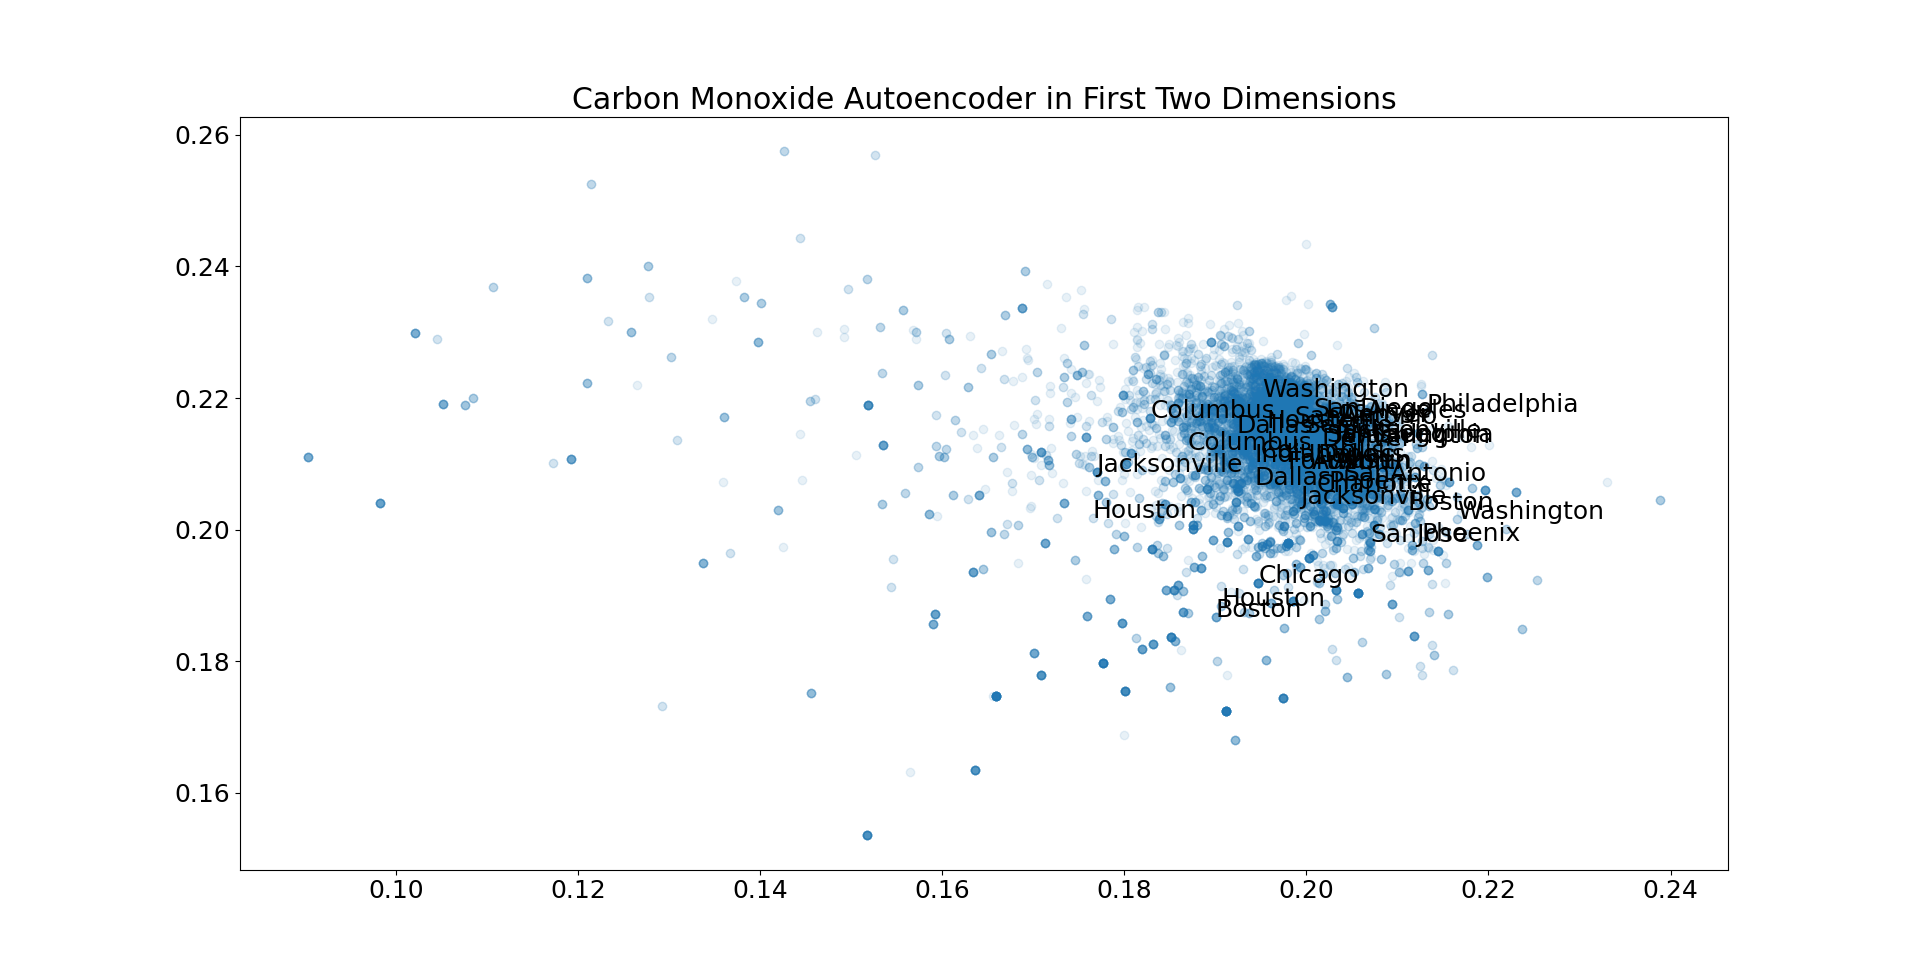
\includegraphics[width=1.1\linewidth, height=5cm]{/home/nicks/github_repos/Pollution-Autoencoders/paper-draft/images/co_scatter_ae_large_cities.png}
    \caption{Densely Populated Cities}
    \label{fig:dense_cities}
\end{subfigure}

\caption{Scatter plots of outlier and highly-populated cities over first two dimensions}
\label{fig:outliers_vs_dense_cities}
\end{figure}

By selecting from a list the top two hundred highly-populated cities, we found that nearly
all of them were located near the center of the clustering. Conversely, we found that many 
of the outliers were smaller cities in rural locations. \par

\newpage

To further explore the meaning of the hidden dimensions, we calculated the Pearson correlation
coefficient of the normalized timeseries data and the embeddings. The Pearson correlation
coefficient allows us allows us to observe the strength of the linear correlation between
the encoded and unencoded values. 
\begin{equation*}
    r_{XY}=\frac{cov(X,Y)}{\sigma_{X} \cdot \sigma_{Y}}
\end{equation*}
\textit{Where cov(X,Y) is the covariance between X and Y \\
and $\sigma_{X},\sigma{Y}$ are the standard deviations of X and Y respectively}

\vspace{0.1in}

We calculated the correlation coefficients and created a correlation matrix of the days that had
correlation coefficients of the highest magnitude.\par

% pipeline
\begin{figure}[h]
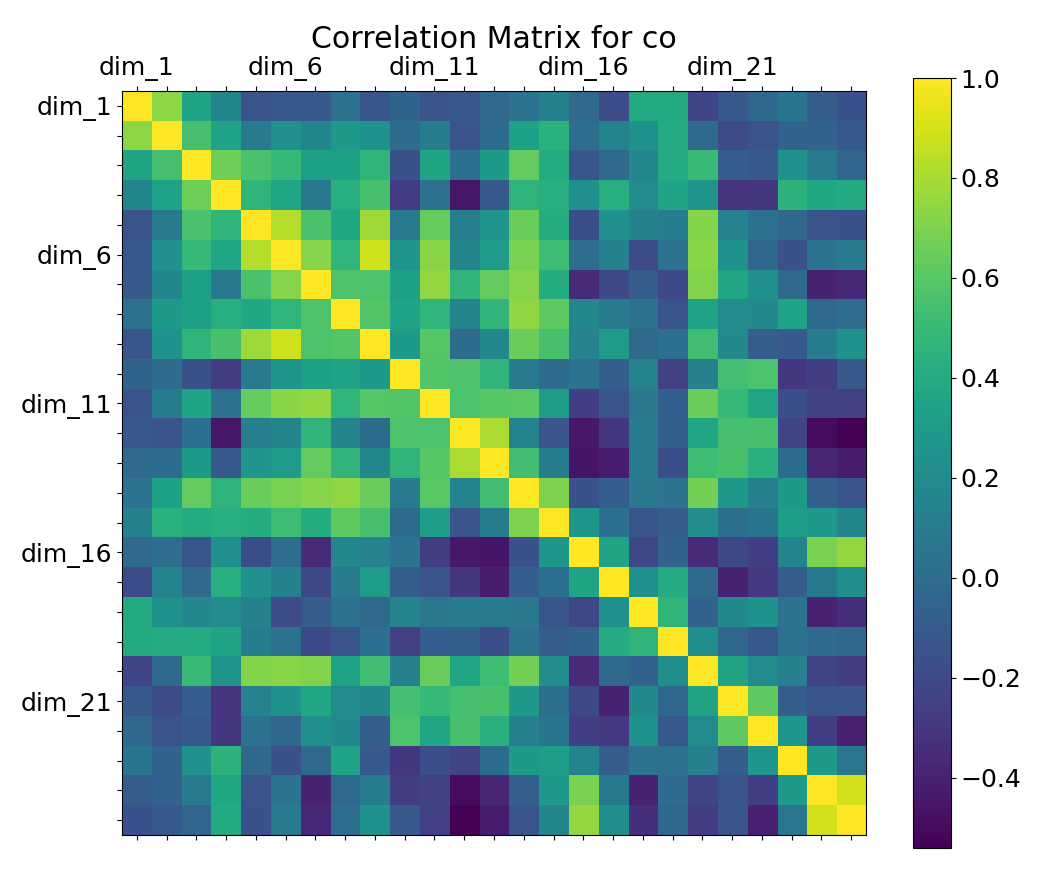
\includegraphics[width=\textwidth]{/home/nicks/github_repos/Pollution-Autoencoders/paper-draft/images/corr_matrix_25.png}
\caption{Correlation Matrix}
\label{fig:matrix}
\end{figure}
\section{Discussion}

\section{Conclusion}

\printbibliography

\end{document}
